\documentclass[a4paper,12pt]{article}
\usepackage[spanish]{babel}
\usepackage[right=2.5cm,left=2.5cm,top=2cm,bottom=2cm]{geometry}
\usepackage[utf8]{inputenc}
\usepackage{amsmath}
\usepackage{amssymb}
\usepackage{mathrsfs}
\usepackage{latexsym}
\usepackage{dsfont}
\usepackage{amsfonts}
\usepackage{array}
\usepackage{hyperref}
%\usepackage{fancyhdr}
\usepackage{xcolor}
%\pagestyle{fancy}
\usepackage{blindtext}
\usepackage{graphicx}
\usepackage{enumerate}
\usepackage{enumitem}
\usepackage{caption}
\usepackage[left]{sidecap}
\usepackage[]{float}
\usepackage{multirow}
\usepackage[style=apa]{biblatex}
\bibliography{bio}



\begin{titlepage}
\centering
{\bfseries\LARGE {Programa en Python\par}
\vspace{1cm}
{\scshape\Large {Proyecto final} \par}
\vspace{3cm}
{\scshape\Huge\textbf {Adivina el Número} \par}
\vspace{3cm}
{\itshape\Large\textbf {Trabajo en equipo}\par}
\vspace{1.5cm}

{\Large\textbf {Members:} \par}

\begin{itemize}
\begin{center}
    \item {\Large{Jared Emmanuel Aguirre Vera}}
    \item {\Large{Luis Fernando Sotomayor Garcia}}
    \item {\Large{Karla Cecilia Valeria Rios Lara}} 
    \item {\Large{Esteban Villa Rosas}}
\end{center}
\end{itemize}
\vspace{6cm}
{\Large December 04, 2022. \par}
\end{titlepage}









\title{Adivina el Número}
\author{Proyecto en equipo }
\date{December 04, 2022}

\begin{document}

\maketitle

\section{Introduction}
\large{Al encontrar diferentes funciones en Python, en este caso nos llamó la atención el poder realizar un programa para un juego divertido, y que hasta cierto punto requiera de un poco de lógica, más adelante se darán cuenta del por qué mencionamos esto.

No obstante, creo que a todos en algún momento nos ha gustado algún juego, pero no siempre sabemos como es que funciona más a detalle, pero durante este proyecto, no solo msotraremos el programa, sino que todo el proceso y lo que se llevo a cabo para ralizarlo de una manera exitosa.}

\section{Hipótesis}
\large{Nuestro objetivo es realizar un programa cuyo propósito sea que una vez que hayamos  dado un número cualquiera, tomando en cuenta que este número debe ser un natural mayor a 1, entonces el  usuario pueda adivinar el número que la computadora elija al azar entre los parametros dados. Donde se le dan indicaciones, de si el número es mayor o menor al número que eligió el usuario y así hasta que pueda llegar al número elejido por la computadora.} 

\section{Metodología}
\large{En primer lugar definimos una función la cual va a tener toda la lógica del programa del juego, y se llamará <adivina\_el\número!, dicha función va a tomar un parámetro el cual se denominara x, este parámetro va a representar el límite superior del intervalo válido de valores. Lo anterior podemos ilustrarlo de la siguiente manera:}


\begin{figure}[H]
    \caption{}
    \centering 
\includegraphics[width=9cm, height=1cm]{funjue.png}
    \label{fig1:my_label}
\end{figure}

\large{Ahora bien, cuando comienza el juego, en proncipio necesitamos mostrar los mensajes de bienvenida al usuario y explicarle cual es la meta del juego, así que haremos esto con la función print, la cual nos permite mostrar un mensaje en la consola al ejecutar el programa. Entonces mostramos el mensaje ¡Bienvenido al juego!.}

\begin{figure}[H]
    \caption{}
    \centering 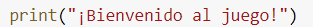
\includegraphics[width=9cm, height=0.7cm]{ba.png}
    \label{fig1:my_label}
\end{figure}

\large{Luego tenemos que mostrar la meta del juego al usuario, mostrando el mensaje ¡el objetivo es adivinar el número generado!}

\begin{figure}[H]
    \caption{}
    \centering 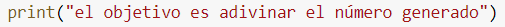
\includegraphics[width=11cm, height=0.8cm]{ob.png}
    \label{fig1:my_label}
\end{figure}

\large{Comenzamos a implementar la funcionalidad del juego generando el número aleatorio, utilizando una sentencia import, la cual nos permite importar un módulo, que es como un archivo que contiene funciones y elementos útiles que podemos usar en nuestro programa. }

\begin{figure}[H]
    \caption{}
    \centering 
\includegraphics[width=9cm, height=1cm]{ir.png}
    \label{fig1:my_label}
\end{figure}

\large{En este caso vamos a importar el módulo ``random'', que significa aleatorio, ya que este nos permite trabajar con procesos aleatorios y pues para nuestro pograma necesitamos generar un número aleatorio y que sea entero, para lo que necesitamos también a la función ``randint'', la cual toma dos parametros a y b pues nos da un intervalo de (a,b), y retorna un entero aleatorio $\mathbb{N}$ tal que $a\leq \mathbb{N} \leq b$, entonces estos parámetros van a determinar
el rango de valores posibles que puede tomar ese valor aleatorio. En este caso definiremos el rango de valores entre 1 y x, esto sería de la siguiente manera.}

\begin{figure}[H]
    \caption{}
    \centering 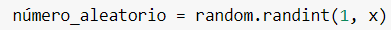
\includegraphics[width=9cm, height=1cm]{nua.png}
    \label{fig1:my_label}
\end{figure}

\large{Llegando hasta aquí debemos implementar la lógica principal del juego. Así, una vez teniendo nuestro número aleatorio, tenemos que preguntarle al usuario que número va a predecir, que es el número aleatorio de la computadora, es por eso que vamos a crear una variable que se va a llamar ``predicción'', de la cual su valor inicial va a ser 0 para que no haya ninguna posibilidad de que coincida inicialmente con el número aleatorio, por ejemplo si nosotros comenzaramos nuestra prediddión con el número uno, puede ser que el número aleatorio también sea uno y la predicción inicial sea uno y entonces no habría juego, el usuario no tendría ni una sola ronda para adivinar el valor.}

\begin{figure}[H]
    \caption{}
    \centering 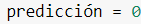
\includegraphics[width=5cm, height=0.8cm]{pre.png}
    \label{fig1:my_label}
\end{figure}

\large{Luego de que definieramos nuestra variable predicción, tenemos que crear una parte repetitiva del proceso, y para ello vamos a utilizar un ciclo ``while'' ya que necesitamos repetir una secuencia de instrucciones, un número no específico de veces, pues nosotros no sabemos cuantas veces tendremos que pedirle al usuario que de una predicción del número, porque el usuario puede adivinar el número a la primera vez o quizá se necesitan 500 repeticiones para llegar al número aleatorio, dependiendo también del tamaño del intervalo.} 

\begin{figure}[H]
    \caption{}
    \centering 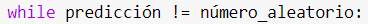
\includegraphics[width=8cm, height=0.8cm]{wh.png}
    \label{fig1:my_label}
\end{figure}

\large{La condición para que el proceso siga es que mientras la predicción no sea igual que el número aleatorio, pues si es igual entonces ya el usuario predijo el número aleatorio correctamente y el juego termina. Por otro lado si la predicción es distinta del número aleatorio entonces necesitamos realizar un proceso específico.}

\begin{enumerate}
    
    \item \large{Primero tenemos que pedirle al usuario que adivine un número entre 1 y x. Para obtener un valor del usuario necesitamos usar la función input, que nos permite interactuar con el usuario, es decir, mostrar un mensaje en el que solicias algo y recibir algo a cambio. Cabe mencionar   que int nos permite transformar el valor ingresado por el usuario a un entero, o mejor dicho, ese valor se asigna como un entero a la variable, permitiendo trabajar bien al programa. Esto nos quedaría de la siguiente manera:}
    
    \begin{figure}[H]
    \caption{}
    \centering 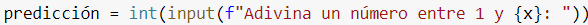
\includegraphics[width=11cm, height=0.7cm]{int.png}
    \label{fig1:my_label}
    \end{figure}
    
    \item \large{Una vez que tenemos la predicción, si la predicción es correcta el ciclo se va a detener, por la condición va a ser falsa. Entonces el jugador gana el juego.}

    
    \item \large{Ahora bien, si la predicción es menor que el número aleatorio, entonces mostramos el mensaje ¡fallaste, intenta con un número más grande!.}

    \begin{figure}[H]
    \caption{}
    \centering 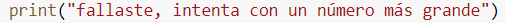
\includegraphics[width=11cm, height=0.6cm]{print1.png}
    \label{fig1:my_label}
    \end{figure}    
    
    \item \large{En cambio, si la predicción es mayor que el número aleatorio, entonces mostramos el mensaje ¡fallaste, intenta con un número más pequeño!}

    \begin{figure}[H]
    \caption{}
    \centering 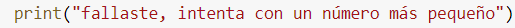
\includegraphics[width=11cm, height=0.7cm]{print2.png}
    \label{fig1:my_label}
    \end{figure}  
    
    \item \large{Finalmente, como se dijo en (2) si la predicción es igual que el número aleatorio, el ciclo se va a detener inmediatamente, cuando esto pase, mostraremos el siguiente mensaje {¡Muy bien! haz hallado el numero {número_aleatorio}. Felicidades}.}

    \begin{figure}[H]
    \caption{}
    \centering 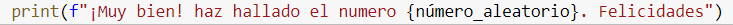
\includegraphics[width=13cm, height=0.7cm]{print3.png}
    \label{fig1:my_label}
    \end{figure}  
    
\end{enumerate}  

\large{Nuestro programa completo quedaría de la siguiente manera.}

    \begin{figure}[H]
    \caption{}
    \centering 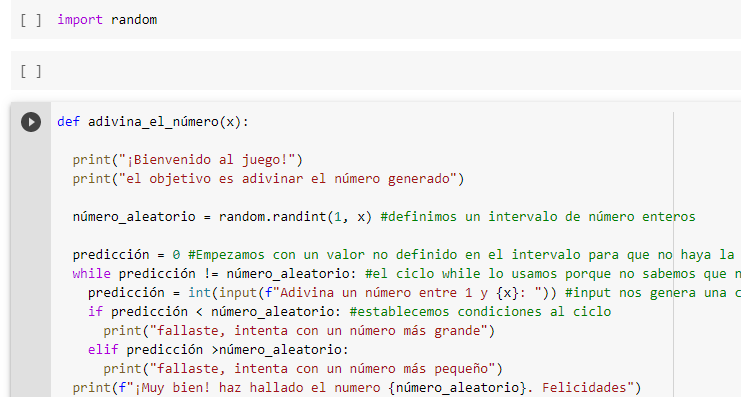
\includegraphics[width=14cm, height=9cm]{pro.png}
    \label{fig1:my_label}
    \end{figure}  

\large{Ahora, para ver funcionar el juego, llamamos a la función, escribiendo el nombre de la función y entre parentesis vamos a pasar el valor de x, en este caso escogimos $x=100$, entonces el funcionamiento del juego sería algo así:}

    \begin{figure}[H]
    \caption{}
    \centering 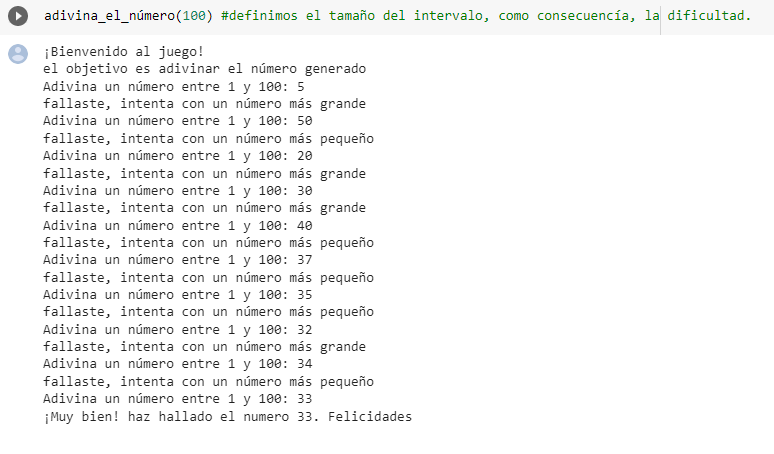
\includegraphics[width=16cm, height=10cm]{ejem.png}
    \label{fig1:my_label}
    \end{figure}  

\section{Resultados}
\large{Pudimos realizar un programa que mediante la definición de unas variables puede hacer un ciclo el cuál se repite hasta obtener un resultado determinado al azar, haciendo que este vaya cambiando cada vez que se ejecute, esto cumple con el hecho de poder servir como un juego, dónde de un conjunto se elije un número al azar y esté debe ser adivinado por el jugador. De esta forma podemos ver como python puede ser usado tanto con fines meramente académicos pero también lúdicos.}

\section{Conclusión}
\large{Pues bien, creo que finalmente, alcanzamos no solamente llegar a nuestro objetivo, sino que durante el proceso, de igual manera seguir aprendiendo de este lenguaje de programación ``Python'', pues si bien en otro momento, por alguna razón ya habíamos visto un poco el como funcionaba estelenguaje, pero pues como bien sabemos, nunca dejamos de aprender, y esto no fué la excepción, ya que, tuvimos que investigar más cosas y relacionarlas con lo que queríamos lograr. Entonces quedamos satisfechos con el proyecto, pues se logró el objetivo y aprendimos nuevas cosas.}


\begin{thebibliography}{}
\bibitem{}. Navone, E. C. (5 de julio de 2021). free code camp. Obtenido de 6 Proyectos de Python Básicos - Curso Completo Paso a Paso: https://youtu.be/tWnyBD2src0

\end{thebibliography}

\end{document}
